% Copyright 2004 by Till Tantau <tantau@users.sourceforge.net>.
%
% In principle, this file can be redistributed and/or modified under
% the terms of the GNU Public License, version 2.
%
% However, this file is supposed to be a template to be modified
% for your own needs. For this reason, if you use this file as a
% template and not specifically distribute it as part of a another
% package/program, I grant the extra permission to freely copy and
% modify this file as you see fit and even to delete this copyright
% notice. 

\documentclass{beamer}

% There are many different themes available for Beamer. A comprehensive
% list with examples is given here:
% http://deic.uab.es/~iblanes/beamer_gallery/index_by_theme.html
% You can uncomment the themes below if you would like to use a different
% one:
%\usetheme{AnnArbor}
%\usetheme{Antibes}
%\usetheme{Bergen}
%\usetheme{Berkeley}
%\usetheme{Berlin}
%\usetheme{Boadilla}
%\usetheme{boxes}
%\usetheme{CambridgeUS}
%\usetheme{Copenhagen}
%\usetheme{Darmstadt}
%\usetheme{default}
%\usetheme{Frankfurt}
%\usetheme{Goettingen}
%\usetheme{Hannover}
%\usetheme{Ilmenau}
%\usetheme{JuanLesPins}
%\usetheme{Luebeck}
\usetheme{Madrid}
%\usetheme{Malmoe}
%\usetheme{Marburg}
%\usetheme{Montpellier}
%\usetheme{PaloAlto}
%\usetheme{Pittsburgh}
%\usetheme{Rochester}
%\usetheme{Singapore}
%\usetheme{Szeged}
%\usetheme{Warsaw}
\usepackage{mathtools}
\usepackage{physics}
\usepackage{graphicx}
\usepackage{varwidth}
\usepackage{float}
\usepackage[utf8]{inputenc}
\usepackage[spanish]{babel}
\usepackage{csquotes}
\usepackage{hyperref}
\usepackage{multicol}
\usepackage{amsmath}
\usepackage[lined]{algorithm2e}
\hypersetup{
    %colorlinks=true,
    %linkcolor=blue,
    filecolor=magenta,      
    urlcolor=cyan,
}
\title{Investigation into the applicability of Grover's Algorithm to search problems}

% A subtitle is optional and this may be deleted
 %\subtitle{Optional Subtitle}

\author{S. Al Hashemi }
% - Give the names in the same order as the appear in the paper.
% - Use the \inst{?} command only if the authors have different
%   affiliation.

\institute[University of Toronto] % (optional, but mostly needed)
{
  Engineering Science\\[1cm]{\small Supervisor: Prof. G. Gulak}
}
% - Use the \inst command only if there are several affiliations.
% - Keep it simple, no one is interested in your street address.

\date{April 2019}
% - Either use conference name or its abbreviation.
% - Not really informative to the audience, more for people (including
%   yourself) who are reading the slides online

% \subject{Theoretical Computer Science}
% This is only inserted into the PDF information catalog. Can be left
% out. 

% If you have a file called "university-logo-filename.xxx", where xxx
% is a graphic format that can be processed by latex or pdflatex,
% resp., then you can add a logo as follows:

% \pgfdeclareimage[height=0.5cm]{university-logo}{university-logo-filename}
% \logo{\pgfuseimage{university-logo}}

% Delete this, if you do not want the table of contents to pop up at
% the beginning of each subsection:
% \AtBeginSubsection[]
%{
  %\begin{frame}<beamer>{Outline}
    %\tableofcontents[currentsection,currentsubsection]
  %\end{frame}
%}

% Let's get started
\begin{document}

\begin{frame}
	\titlepage
\end{frame}

\begin{frame}{Outline}
	\tableofcontents
	% You might wish to add the option [pausesections]
\end{frame}

% Section and subsections will appear in the presentation overview
% and table of contents.
\section{Introduction to Quantum Computing}

\begin{frame}{Motivation and Objective}
	\begin{block}{Motivation}
		\begin{multicols}{2}
			\begin{itemize}
				\item Encryption cracking for encryption schemes based on the Shortest Vector Problem (Lattice Schemes).
				\item Fast global optimization of mathmatical functions.
				      %\item Collision problem in complexity theory
			\end{itemize}

			\columnbreak
			\begin{itemize}
				\item Machine Learning
				\item Quantum Chemistry
				\item Searching problems
			\end{itemize}
		\end{multicols}
	\end{block}
	\begin{exampleblock}{Objective}
		\begin{itemize}
			\item Gain insight into the hardware requirements necessary to implement Grover's algorithm.
			\item Develop test quantum circuits for known problems.
		\end{itemize}
	\end{exampleblock}
\end{frame}
\subsection{Quantum Computers}
\begin{frame}{Quantum Computers}
	\begin{itemize}
		\item First proposed by Richard Feynman
		\item {
		      Takes advantage of several quantum theories to solve problems not computable in polynomial time on classical computers.
		      }
		      \begin{itemize}
			      \item \textbf{Superposition} of quantum state
			      \item \textbf{Quantum entanglement} of state
		      \end{itemize}
	\end{itemize}
\end{frame}

\subsection{Comparison with Classical Computing}

\begin{frame}{Comparison with classical computing}
	%\begin{table}[]
	%\centering
	%\resizebox{\columnwidth}{!}{%
	%\begin{tabular}{ll}
	%\textit{Classical}               & \textit{Quantum}                                             \\
	%Built on semiconducting material & Construction depends on model \\
	%Encode information into bits     & Encode information into qubits/qumodes                       \\
	%\textbf{Deterministic}           & \textbf{Non-deterministic}
	%\end{tabular}%
	%}
	%\end{table}
	%\begin{multicols}{2}
	\textbf{Classical Computers}
	\begin{itemize}
		%\item More or less, a single dominant model
		\item Built on semiconducting material (ie.\ silicon)
		\item Encode information into bits which operate by manipulating charge.
		\item \textbf{Deterministic} in nature $\rightarrow$ you can know the state of a bit or a group of bits before any measurement is made.
	\end{itemize}
	%\columnbreak
	\textbf{Quantum Computers}
	\begin{itemize}
		%\item Multiple models exist $\rightarrow$ qubit model/continuous-variable model
		\item Construction depends on the model $\rightarrow$ popular forms of the qubit model are built on superconducting material.
		\item Encode information into qubits/qumodes.
		\item \textbf{Non-deterministic} $\rightarrow$ probabilistic by nature.
	\end{itemize}
	%\end{multicols}
\end{frame}

\subsection{Qubits}

% You can reveal the parts of a slide one at a time
% with the \pause command:
%\begin{frame}{Quantum State}
%\begin{itemize}
%%\item Abstraction of the present/future state of a classical system to a quantum state. It is described by a wavefunction.
%\item Braket notation is used to describe a wavefunction:
%\begin{equation}
%\ket{\Psi} = \sum_i \alpha_i \ket{\psi_i}
%\end{equation}
%\item In order to know the state of the system, the wavefunction must be measured. The coefficients $\alpha_i$ are proportional to the probability of state $\ket{\psi_i}$ being measured.
%%\item We can conceptualize this as `how much of $\ket{\psi_i}$ is in $\ket{\Psi}$`, with the set of $\ket{\psi_i}$'s being the basis for all posible states of a system.
%\item \textbf{Normalization Constraint}: $\sum_i |\alpha_i|^2 = 1$
%\item The vector space the contains all possible states is known as the \textit{Hilbert Space}.
%\end{itemize}
%\end{frame}

\begin{frame}{Qubits}
	\begin{block}{Quantum Basis of Qubits}
		The state of a qubit is naturally described by a discrete basis of ${ \ket{0}, \ket{1}}$ $\rightarrow$ the ground/excited states.
	\end{block}
	\begin{itemize}
		\item The general state of a qubit is thus:
		      \begin{equation}
			      \ket{\Psi} = \alpha \ket{0} + \beta \ket{1}
		      \end{equation}
		\item This can be further represented as:
		      \begin{equation}
			      \ket{\Psi} \rightarrow \begin{bmatrix} \alpha \\ 0  \end{bmatrix} + \begin{bmatrix} 0 \\ \beta \end{bmatrix}
		      \end{equation}
		\item \textbf{Normalization Constraint}: $|\alpha|^2 + |\beta|^2 = 1$
		      %\item The representation of a quantum operator in this basis is generally given by the set of operations that define a matrix:
		      %\begin{equation}
		      %A \rightarrow \begin{bmatrix} \bra{0}A\ket{0} & \bra{0}A\ket{1} \\ \bra{1}A\ket{0} & \bra{1}A\ket{1} \end{bmatrix}
		      %      \end{equation}
	\end{itemize}
	\begin{figure}[Measurement of a qubit]
		\centering
		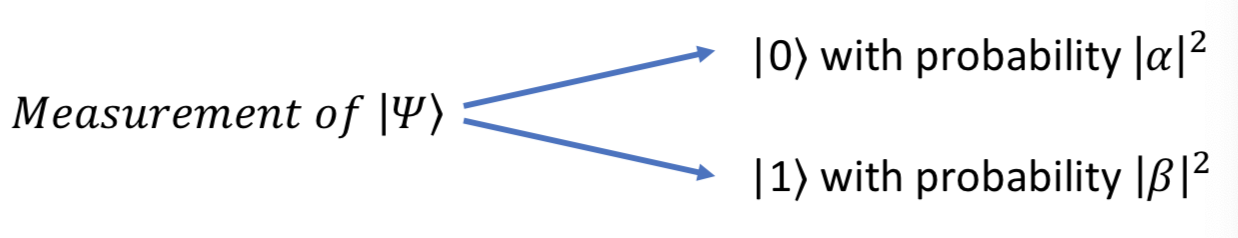
\includegraphics[scale=.3]{./measurement.png}
	\end{figure}

\end{frame}

%\begin{frame}{Bloch Sphere}
%\begin{block}{Quantum Basis of Quabits}
%The qubit's state can be interpreted as living in the \textit{Bloch Sphere}, a 2-basis abstraction of the Hilbert Space.
%\end{block}
%\begin{figure}[H]
%\hspace{1.5cm}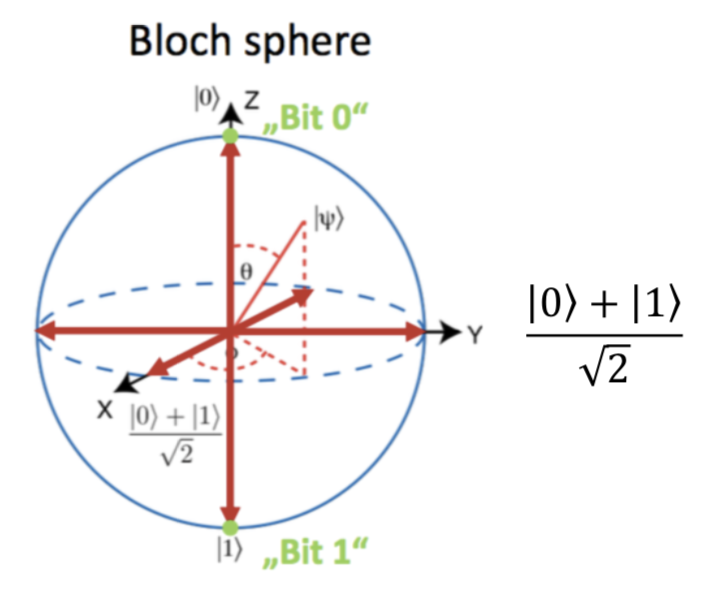
\includegraphics[scale=.5]{bloch.png}
%\end{figure}
%\end{frame}

%\begin{frame}{Measurement}
%\begin{block}{}
%Measurement of a qubit in superposition will collapse a state onto one of its basis vectors.
%\end{block}
%\begin{figure}[Measurement of a qubit]
%\centering
%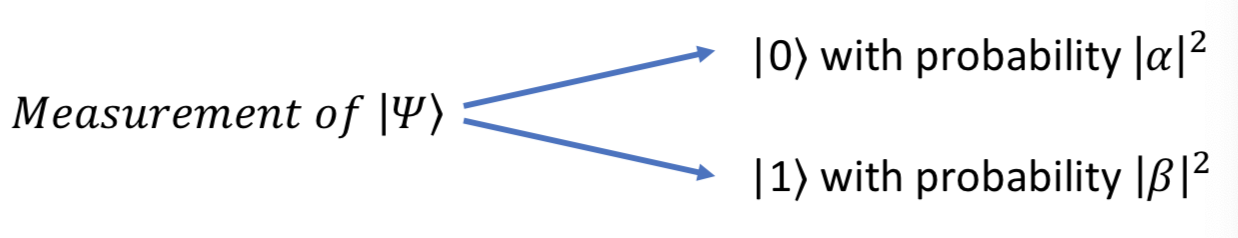
\includegraphics[scale=.5]{./measurement.png}
%\end{figure}
%\end{frame}


%\begin{frame}{Coherence of Qubits}
%\begin{block}{Quantum Basis of Quabits}
%It is important that qubits maintain constant phase relations within the Bloch Sphere.
%\end{block}
%\begin{figure}[H]
%\hspace{.8cm}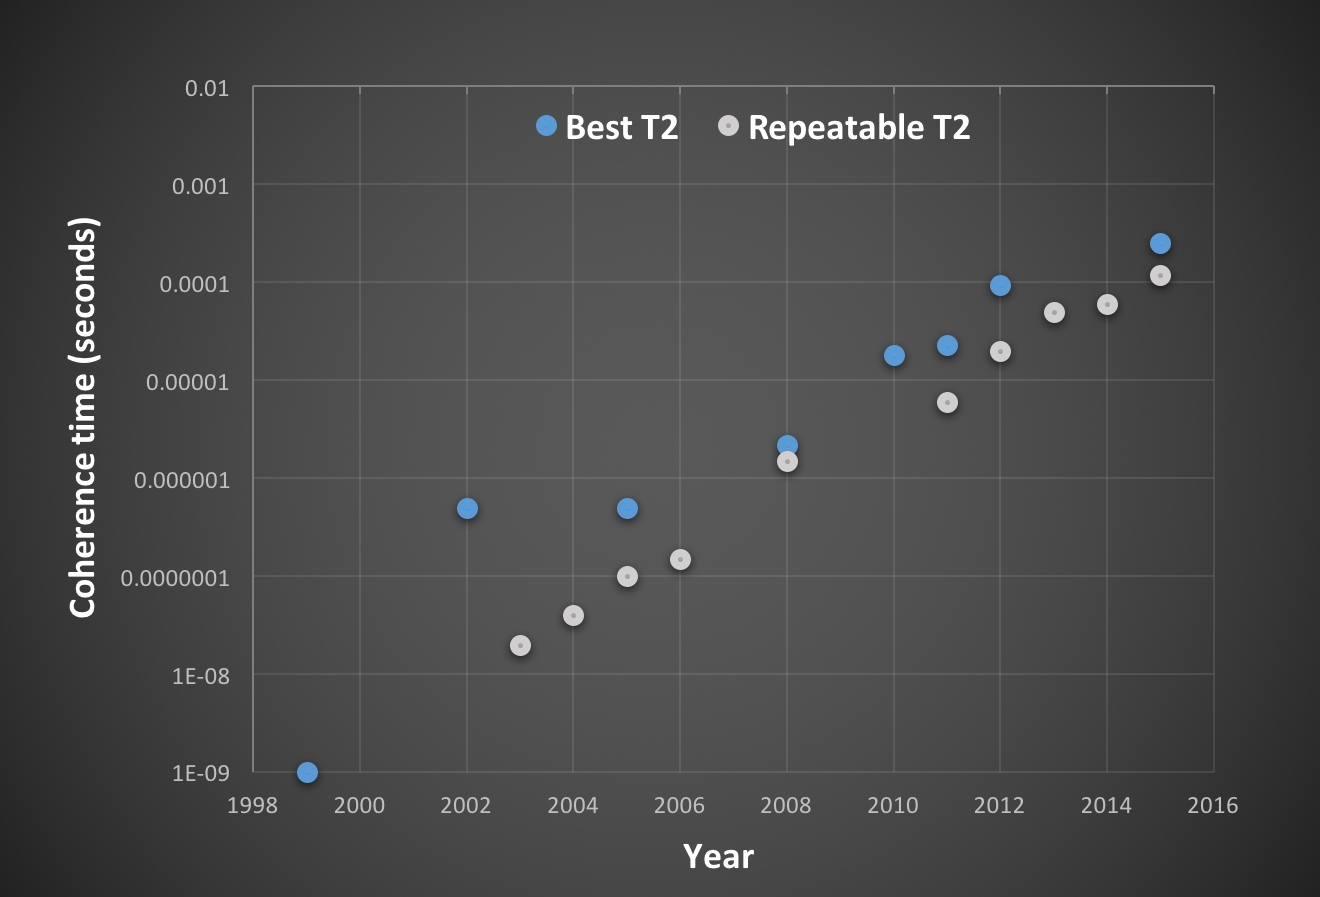
\includegraphics[scale=.36]{./IBMQ_coherence.png}
%\end{figure}
%\end{frame}


\subsection{Quantum Circuits}
\begin{frame}{Quantum Gates}
	\begin{block}{Quantum Gates}
		\begin{itemize}
			\item Unitary operations that modify the state of a qubit(s)
			\item Must preserve probability amplitudes normalization.
		\end{itemize}
	\end{block}
	\begin{table}[]
		\begin{tabular}{|l|l|}
			\hline
			\textit{NOT Gate}                                                             & \textit{HADAMARD Gate}                                                                                                                          \\ \hline
			\textit{} $ X = \begin{bmatrix}
					0 & 1 \\
					1 & 0
				\end{bmatrix}  $                                 & $H = \frac{1}{\sqrt{2}} \begin{bmatrix}
					1 & 1  \\
					1 & -1
				\end{bmatrix}$\textit{}                                                                                    \\ \hline
			$X\ket{0} = \begin{bmatrix}
					0 & 1 \\
					1 & 0
				\end{bmatrix} \begin{bmatrix}
					1 \\ 0
				\end{bmatrix} = \ket{1} $ & $H\ket{0}= \frac{1}{\sqrt{2}} \begin{bmatrix}
					1 & 1  \\
					1 & -1
				\end{bmatrix}\begin{bmatrix}
					1 \\ 0
				\end{bmatrix}  $ $= \frac{1}{\sqrt{2}}\ket{0} + \frac{1}{\sqrt{2}}\ket{1}$ \\ \hline
		\end{tabular}
	\end{table}
\end{frame}
%\begin{frame}{Quantum Circuits}
%\begin{itemize}
%\item Conceptually represented by a series of parallel lines that represent a qubit each.
%\item Quantum operations are done with quantum gates, such as $A$ shown previously.
%\begin{block}{Restriction on Gates}
%These gates must be reversible (unitary), as nature restricts that the operator must preserve the information of a system (information cannot be destroyed but transformed).
%\end{block}
%\item Common gates include the $NOT$ gate and the $HADAMARD$ gate.
%\end{itemize}
%\end{frame}

%\begin{frame}{Quantum Circuits}
%\begin{figure}[H]
%\hspace{0cm}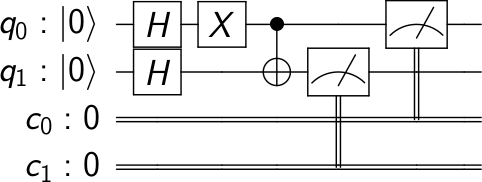
\includegraphics[scale=.36]{./sample_circuit.png}
%\caption{A sample quantum circuit}
%\end{figure}
%\end{frame}

%\begin{frame}{Phase Kickback}
%\begin{itemize}
%\item As quantum computers take advantage of quantum entanglement, there are several unique mechanisms that are not available to classical computers.
%\begin{block}{Phase Kickback}
%Without diving into detail, phase kickback is the explicit operation on one qubit, that implicitly changes the state of another entangled qubit.
%\end{block}
%\end{itemize}
%\end{frame}

\subsection{Time Complexity}
%\begin{frame}{The power of quantum computers}
%\begin{itemize}
%\item Classical computers encode information with bits, which are deterministic and can only hold a value of $0$ or $1$ at a single time.
%\item Qubits, on the other hand, can be any arbitrary state representable on the Bloch Sphere at any time, and only upon measurement will collapse onto one of the basis states $\ket{0}$ or $\ket{1}$.
%\begin{block}{Encoded Information}
%\begin{itemize}
%\item A string of $n$ bits can at an instance can hold at max $n$ $0$'s or $1$'s.
%\item In contrast, a string of $n$ qubits can be at a single time, $2^n$ different permutations; an exponential increase of information.
%\end{itemize}
%\end{block}
%\end{itemize}
%\end{frame}
\begin{frame}{Time Complexity}
	\begin{block}{Quantum Complexity}
		\textit{Bounded-Error Quantum Polynomial Time (BQP)} is a classification for a set of problems that require a polynomial amount of resources on a quantum computer.
	\end{block}
	\begin{figure}[BQP]
		\centering
		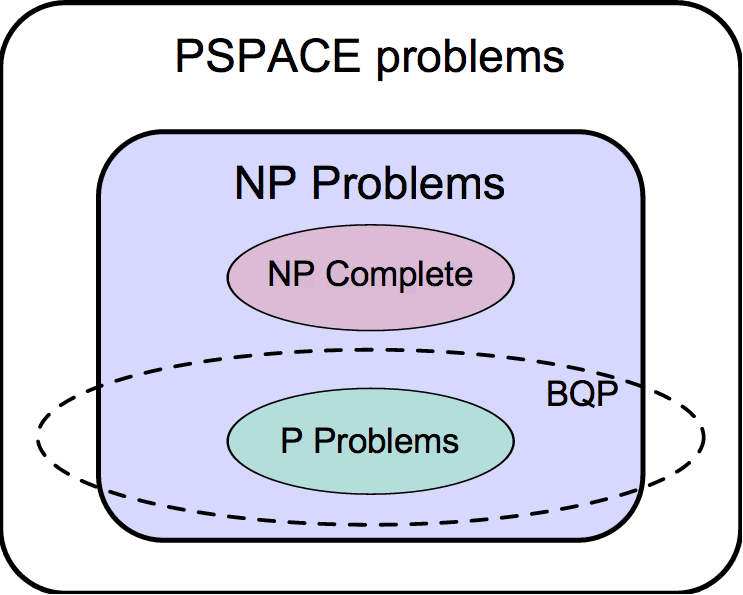
\includegraphics[scale=.24]{./bqp.png}
	\end{figure}
	%\begin{itemize}
	%\item In classical computing, problems are classified as ones that can be computed in polynomial time $(P)$, and those that cannot be, $(NP)$.
	%\item This is one reason Feynman came up with the idea of a quantum computer, as he realized some problems require the ability to encode an exponential amount of information.
	%\begin{itemize}
	%\item For example, simulation of quantum particles.
	%\end{itemize}
	%\item Computational complexities ara also defined for quantum computation.
	%\end{itemize}
\end{frame}

\section{Grover's Algorithm}

\subsection{Problem Statement}

\begin{frame}{Grover's Algorithm}
	% block, theorem, example are available
	\begin{block}{Problem Statement}
		Given an input space $X_n = \{x_0, x_1, x_2, \ldots, x_n\}$ to an oracle function, $f(x) \rightarrow \{1, 0\}$ it is the goal of the algorithm to find the target element $x^*$ such that $f(x^*) = 1$
	\end{block}
	%\begin{itemize}
	%\item This problem can be conceptualized into an \textit{unstructured search} in a function space.
	%\end{itemize}
	\begin{figure}[Simple Grover]
		\centering
		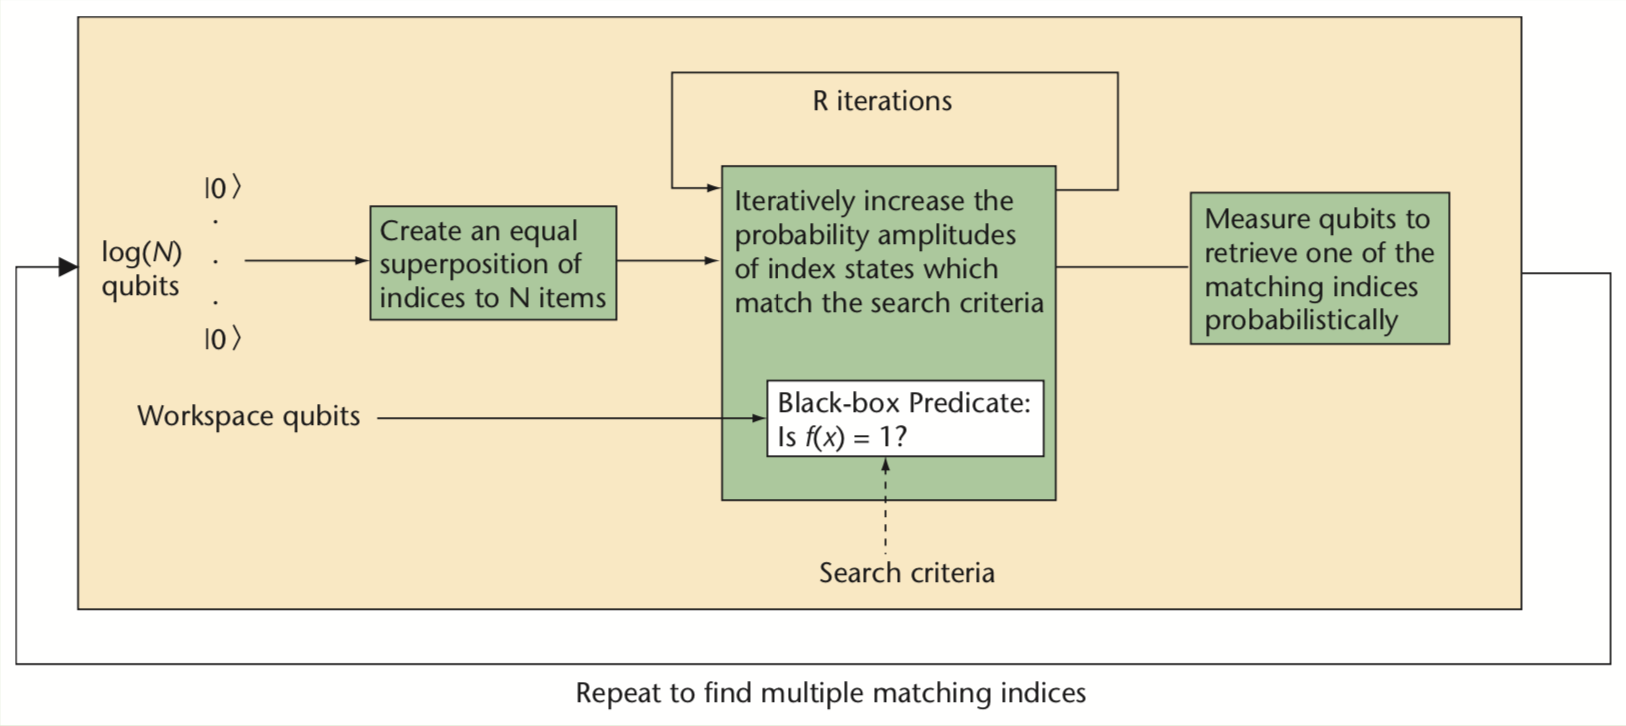
\includegraphics[scale=.4]{./simple_grovers.png}
	\end{figure}
\end{frame}


%\begin{frame}{Classical Unstructured Search}
%In order to find an element in an unsorted list with unique elements (analog to a function space) classically, there are few ways to proceed:
%\begin{itemize}
%\item Cycle through each element, one by one, until you find an element that satifies what you were searching for. $O(n)$
%\item Sort the list first, and then search with knowledge that the list is sorted. $O(nlogn)$
%\end{itemize}

%\begin{block}{Classical Time Bound}
%\begin{itemize}
%\item The classical search for a satisfactory solution thus can at minimum be $O(n)$, where $n$ can vary depending on the search space.
%\item For example, for the 3-SAT problem, $n$ is exponential.
%\item 3-SAT os defined, classically, as \textit{NP-hard}.
%\end{itemize}
%\end{block}
%\end{frame}

%\begin{frame}{Idealized Advantages}
%\begin{block}{Comparison vs. Classical Solutions}
%\begin{itemize}
%\item As discussed, classical solution's time complexity is bounded $O(n)$
%\item Grover's algorithm can ideally solve for the unique answer in time $O(\sqrt{n})$.
%\end{itemize}
%\end{block}
%\end{frame}


%\begin{frame}{Grover's Oracle Function}
%%\begin{itemize}
%%\item In order for Grover's algorithm to proceed, an Oracle function must be given.
%%\item The purpose of the Oracle is to check whether an input in the function space meets the criterion of the given search.
%%\item Referring back to the problem statement, the Oracle would be the function, $f(x)$, which takes an input, $x$, encoded as an $n-bit$ string.
%%\end{itemize}
%\begin{block}{Oracle Function}
%For each function space to query, an Oracle function that acts as a black box must be given to check whether a unique member of the function space satisfies the search criterion.
%\end{block}
%\begin{exampleblock}{Problem}
%This requires that each application of Grover's requires a new Oracle to be constructed.
%\end{exampleblock}
%\end{frame}

\subsection{Breakdown of Grover's Algorithm}
\begin{frame}{Components of Grover's Algorithm}
	\begin{block}{Breakdown}
		\begin{multicols}{2}
			\begin{itemize}
				\item The Oracle query step, $O_f$
				\item Amplitude Amplification, $D$
			\end{itemize}

			\columnbreak
			\scalebox{.7}{                        %new code
				\begin{algorithm}[H]              %new code
					\DontPrintSemicolon
					Initialize equal superposition of states
					\For{i in range($\sqrt{N}$)}{
						Perform Oracle Query
						Apply Diffusion Operator
					}
				\end{algorithm}
			}
		\end{multicols}
	\end{block}
	\begin{figure}[Block representation of Grover's Circuit]
		\centering
		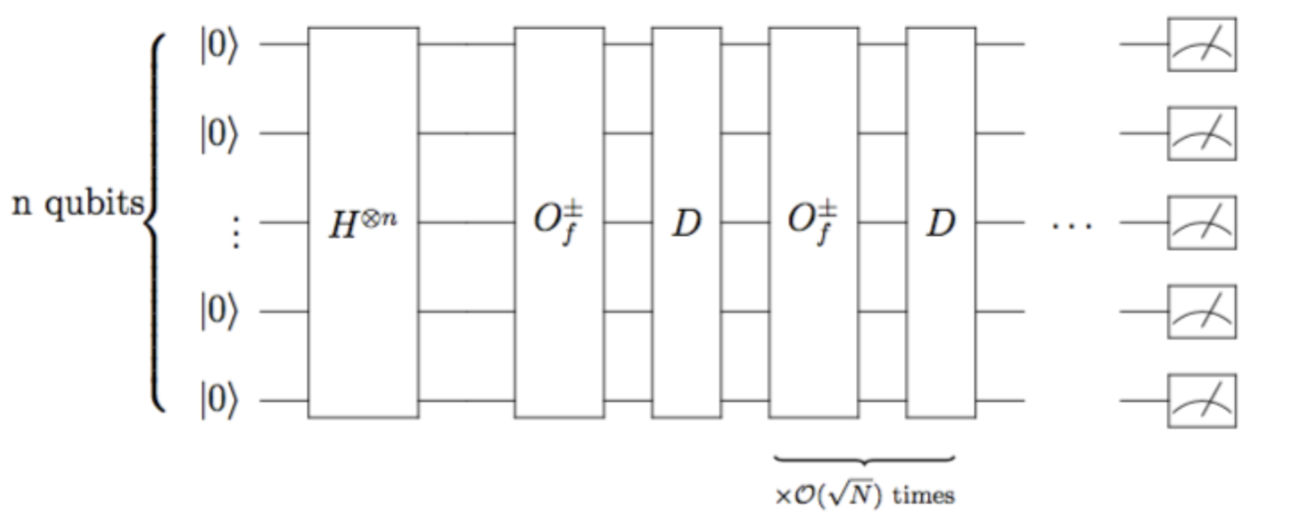
\includegraphics[scale=0.5]{./grover_block.png}
	\end{figure}

\end{frame}

\begin{frame}{Oracle Query}
	\begin{itemize}
		\item It's easy to say that there is a need to have a function that distinguishes between good and bad inputs, s.t.\ for a unique input $x^*$, $f(x^*)=1$, but how is this accomplished on a quantum computer?
		\item An input that satisfies the search criterion can have its phase amplitude, $\alpha_i$ flipped. That is:
		      \begin{equation}
			      \alpha_i \rightarrow -\alpha_i
		      \end{equation}
	\end{itemize}
\end{frame}

%\begin{frame}{Oracle Query}
%%\begin{itemize}
%%\item This can be done by applying $CONTROL-NOT$ gates to the qubits and hitting an extra target qubit with a $Z$ gate, which flips the phase of a qubit.
%%\item This is an example of \textit{phase kickback}.
%%\end{itemize}
%\begin{center}
%A constructed oracle for the function $f(x==111)$
%\end{center}
%\begin{figure}[Oracle for 111]
%\centering
%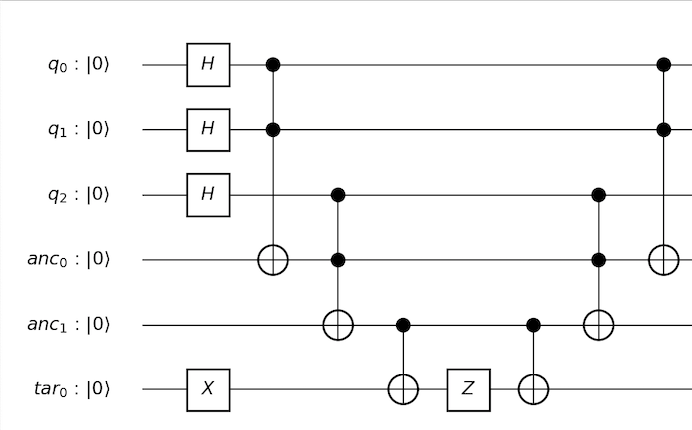
\includegraphics[scale=0.5]{./first_oracle_broken.png}
%\end{figure}
%\end{frame}


\begin{frame}{Grover's Diffusion Gate}
	\begin{block}{Amplitude Amplification}
		Grover's Diffusion Gate applies this mapping:
		\begin{equation}
			\alpha_x\ket{x} \rightarrow (2\mu - \alpha_x)\ket{x}
		\end{equation}
		Here, $\mu=\frac{1}{N}\sum_x\alpha_x \forall x\in\{0, 1\}^n$
	\end{block}
	\begin{itemize}
		\item Recall that the Oracle query operation flips the phase of the state's normalized amplitude: $\alpha_x \rightarrow -\alpha_x$.
		\item The first application of the Oracle gives $\mu = \frac{1}{N}(\frac{N-1}{\sqrt{N}} + \frac{1}{\sqrt{N}}) \approx \frac{1}{\sqrt{N}}$
	\end{itemize}
\end{frame}

\begin{frame}{Grover's Diffusion Gate}
	\begin{block}{Diffusion Gate Mapping}
		The result of this mapping will thus be:
		\begin{itemize}
			\item For positive amplitudes:
			      \[
				      \frac{1}{N} \rightarrow (\frac{2}{\sqrt{N}} - \frac{1}{\sqrt{N}}) = \frac{1}{\sqrt{N}}
			      \]
			\item For the flipped amplitude:
			      \[
				      -\frac{1}{N} \rightarrow (\frac{2}{\sqrt{N}} + \frac{1}{\sqrt{N}}) = \frac{3}{\sqrt{N}}
			      \]
		\end{itemize}
		The amplitude of the marked (flipped) state increases! Grover's algorithm requires $\sqrt{N}$ operations, before the marked state reaches a probability amplitude such that the correct state will \textit{almost certainly} be measured.
	\end{block}
\end{frame}

\begin{frame}{Compilation Time and Problem Size}
	\begin{block}{Problem Size}
		\begin{itemize}
			\item If items in the function space need $n$ bits to be encoded, Grover's Algorithm requires approximately $2n$ qubits.
			\item Depending on the problem at hand, an exponential number of quantum gates (in $n$) are required.

		\end{itemize}
	\end{block}
\end{frame}

\section{Simple Implementations of Grover's Algorithm}

\subsection{Applied to SAT}
\begin{frame}{Satisfiability Application}
	\begin{center}
		This is the full circuit for the problem considered earlier with the search criterion $f(x==111)$.
	\end{center}
	\begin{figure}[Satisfiability 111]
		\centering
		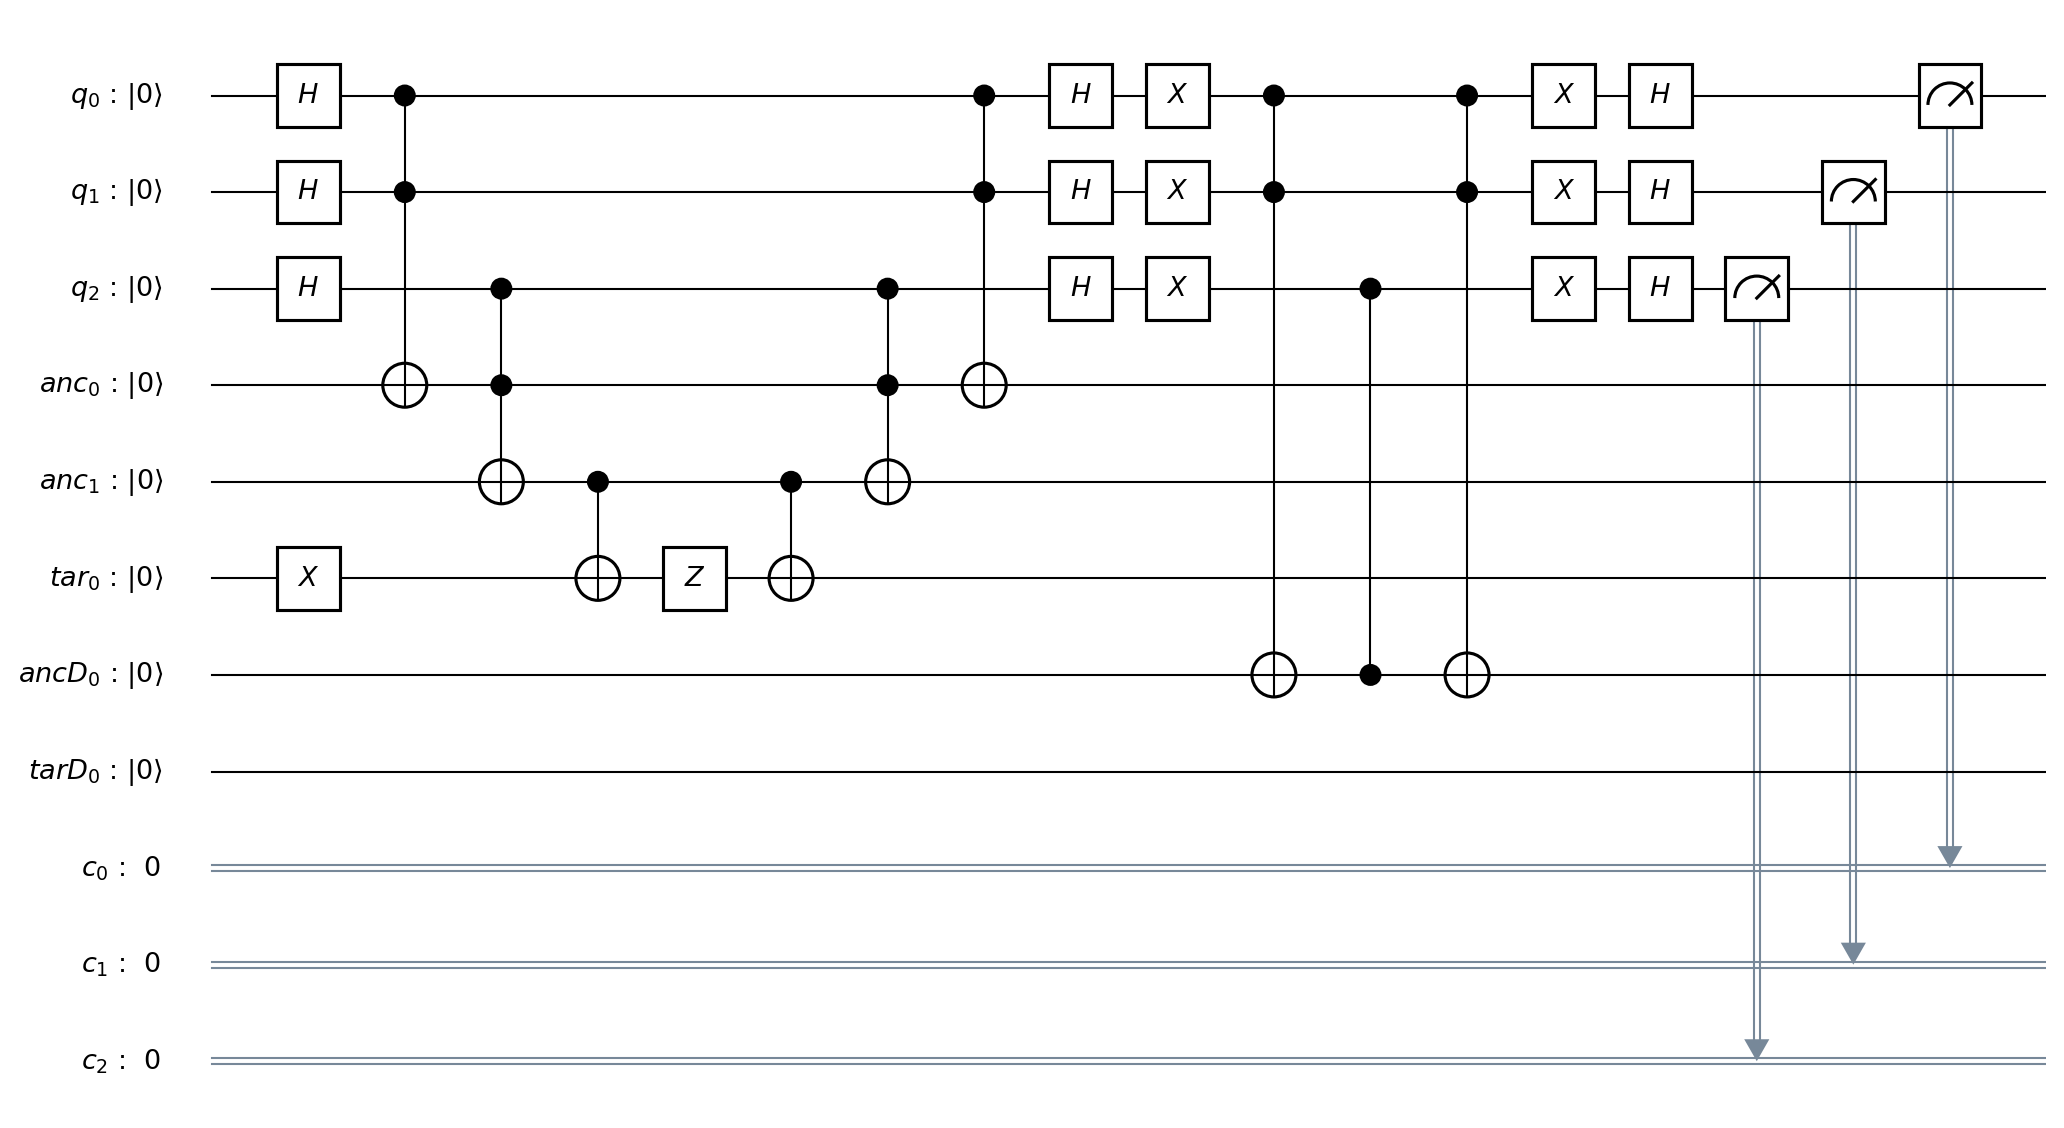
\includegraphics[scale=.3]{./gidney3_class.png}
		%\caption{Complete Grover's Circuit for the search criterion $f(x==111)$}
	\end{figure}
\end{frame}

\begin{frame}{Satisfiability Application}
	\begin{center}
		Histogram of Satisfiability measurements
	\end{center}
	\begin{figure}[Histogram of Satisfiability measurements]
		\centering
		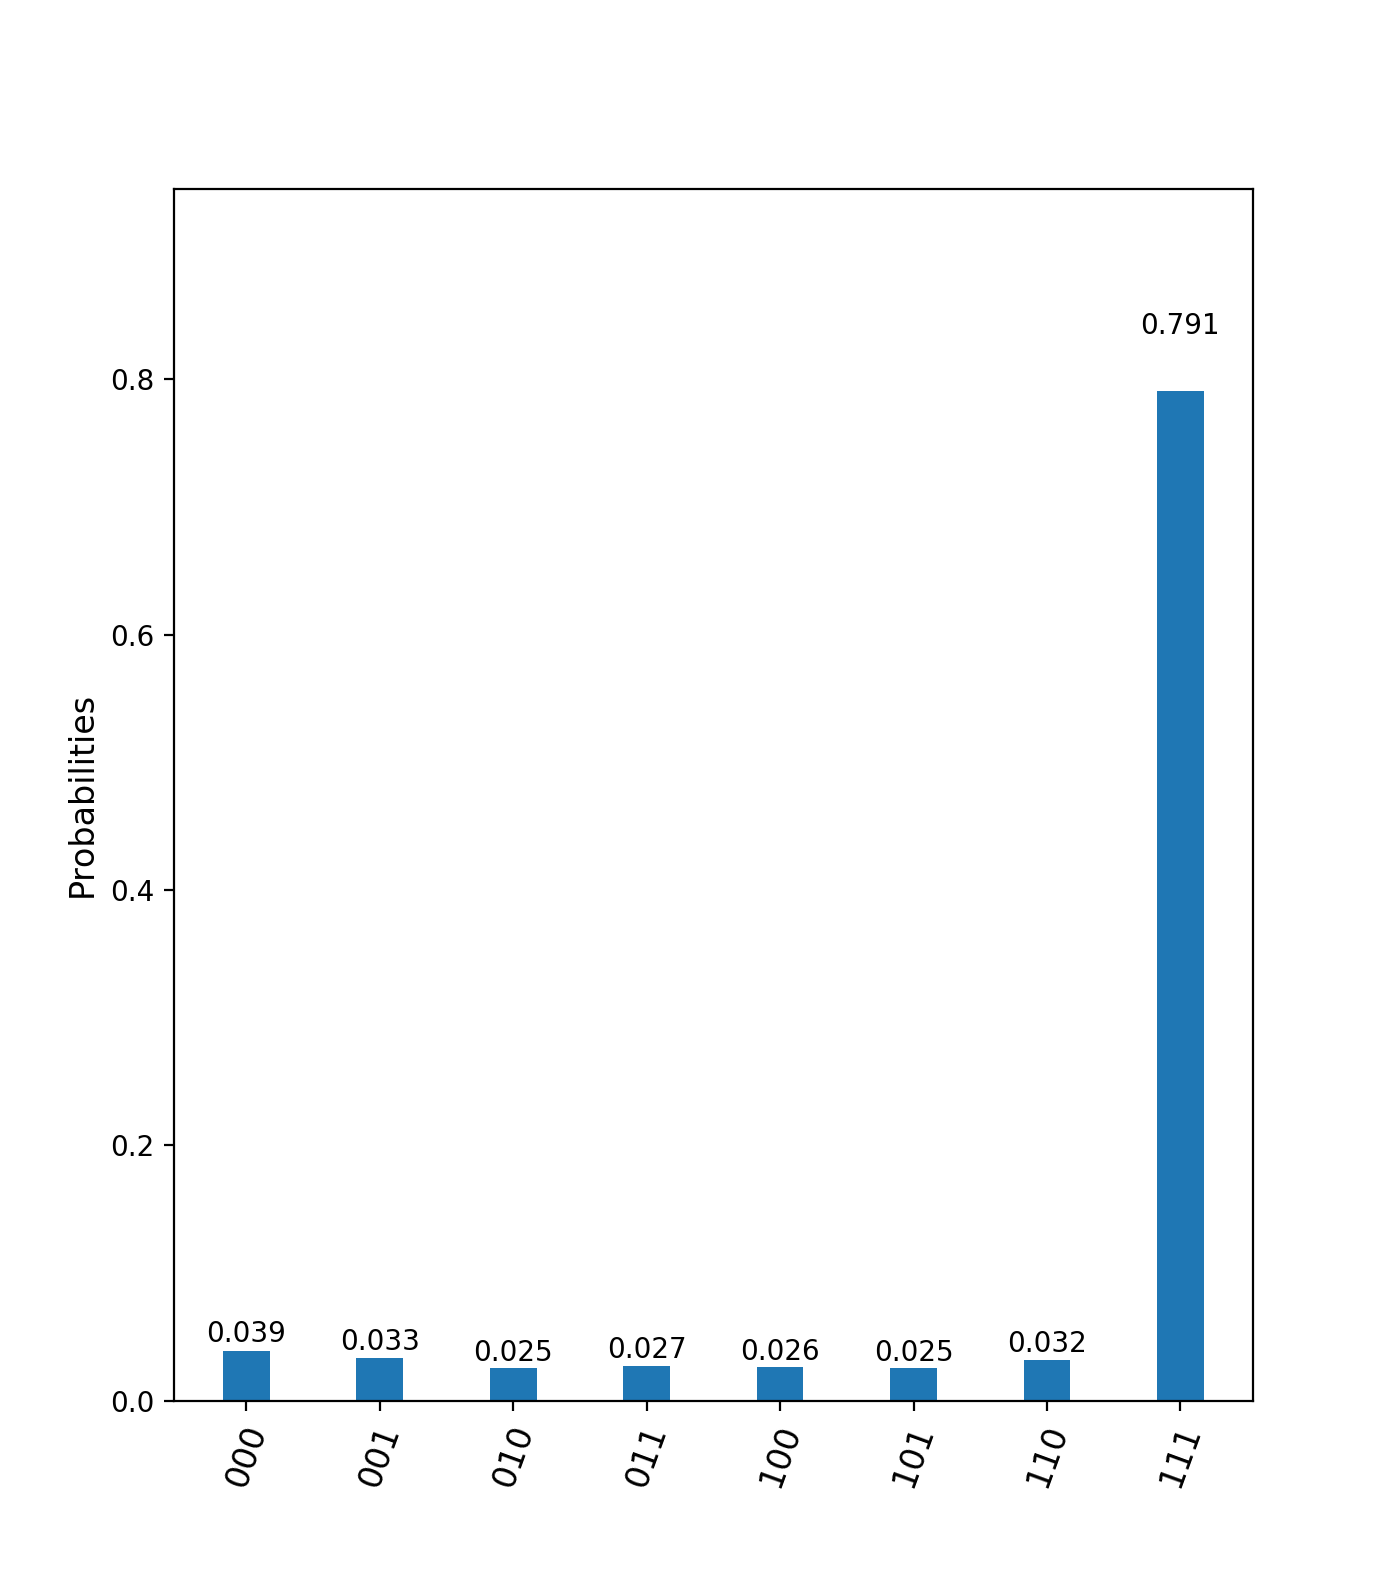
\includegraphics[scale=.34]{./111_histogram.png}
	\end{figure}
\end{frame}


%\subsection{Deficiencies with Grover's Algorithm}


\begin{frame}{Conclusions}
	\begin{itemize}
		\item Quantum hardware is available and readily tested on, however major challenges are still available for Grover's algorithm to be applicable.
		\item Grover's Algorithm can succesfully solve an unstructured search in a function space, given a constructed oracle, faster than any classical methodology.
		\item If practical, Grover's Algorithm presents a threat to all Lattice-based encryption schemes.
	\end{itemize}
\end{frame}

\begin{frame}{Further Work}
	\begin{itemize}
		\item Investigate the scalability of the Oracle; can it be implemented for simple problems without using an extra amount of qubits and quantum gates?
		\item Grover's algorithm assumes the oracle is given, so for each new quantum search a new one must be constructed.
		      \begin{itemize}
			      \item Can an oracle be built that probabilistically encodes classes of search problems?
		      \end{itemize}
	\end{itemize}
\end{frame}


\begin{frame}{Further Reading}
	\begin{block}{Resources}
		\begin{itemize}
			\item L. Grover, 'A fast quantum mechanical algorithm for database search,' \textit{arXiv:quant- ph/9605043, 1996.}
			\item T. Laarhoven, M. Mosca, and J. V. D. Pol, “Solving the Shortest Vector Problem in Lattices Faster Using Quantum Search,” \textit{Post-Quantum Cryptography Lecture Notes in Computer Science}, vol. 1, no. 6176, pp. 83–101, Jan. 2013.
			\item Baritompa, William \& W. Bulger, D \& Wood, Graham. (2005). Grover's Quantum Algorithm Applied to Global Optimization. SIAM Journal on Optimization. 15. 1170-1184. 10.1137/040605072.
		\end{itemize}
	\end{block}
\end{frame}


\begin{frame}{Questions?}
	\begin{figure}[]
		\centering
		
\includegraphics[scale=1]{./question.png}
	\end{figure}
\end{frame}

\begin{frame}{Compilation Time and Problem Size}
	\begin{block}{Quote from Craig Gidney from Google's Quantum Computing}
		\begin{displayquote}
			The actual obstacle to running Grover's algorithm in practice is that the circuits are large, so you need error correction, but this adds significant overhead. Evaluating a function under superposition is easily a billion times less energy efficient than classically computing the same function, using current techniques. This requires you to go to absolutely enormous problem sizes in order for the quadratic advantage to overcome this starting penalty, and because Grover search cannot be paralelized the result is a quantum circuit that will take on the order of a year or a decade to evaluate. There are not very many problems where people would be willing to wait ten years to make the computation 10x cheaper, in terms of dollars, compared to running in parallel on a hundred thousand cloud computers for a few weeks.
		\end{displayquote}
	\end{block}
\end{frame}

%\subsection{Applied to 3-SAT}
\begin{frame}{3-SAT Application}
	\begin{block}{3-SAT Problem}
		The following is an application for the 3-SAT
		\[
			\begin{matrix}
				(\neg x1 \wedge \neg x3 \wedge \neg x4) \vee \\
				(x2 \wedge x3 \wedge \neg x4) \vee           \\
				(x1 \wedge \neg x2 \wedge x4) \vee           \\
				(x1 \wedge x3 \wedge x4) \vee                \\
				(\neg x1 \wedge x2 \wedge \neg x3)
			\end{matrix}
		\]
		\url{https://firebasestorage.googleapis.com/v0/b/arduinohandler.appspot.com/o/Photos\%2F3SAT.png?alt=media\&token=ca052733-38ef-450e-bfd4-024bbb62d7d3}
	\end{block}
\end{frame}


\begin{frame}{3-SAT Application}
	\begin{center}
		Resulting histogram of measured counts
	\end{center}
	\begin{figure}[Resulting histogram of measured counts]
		\centering
		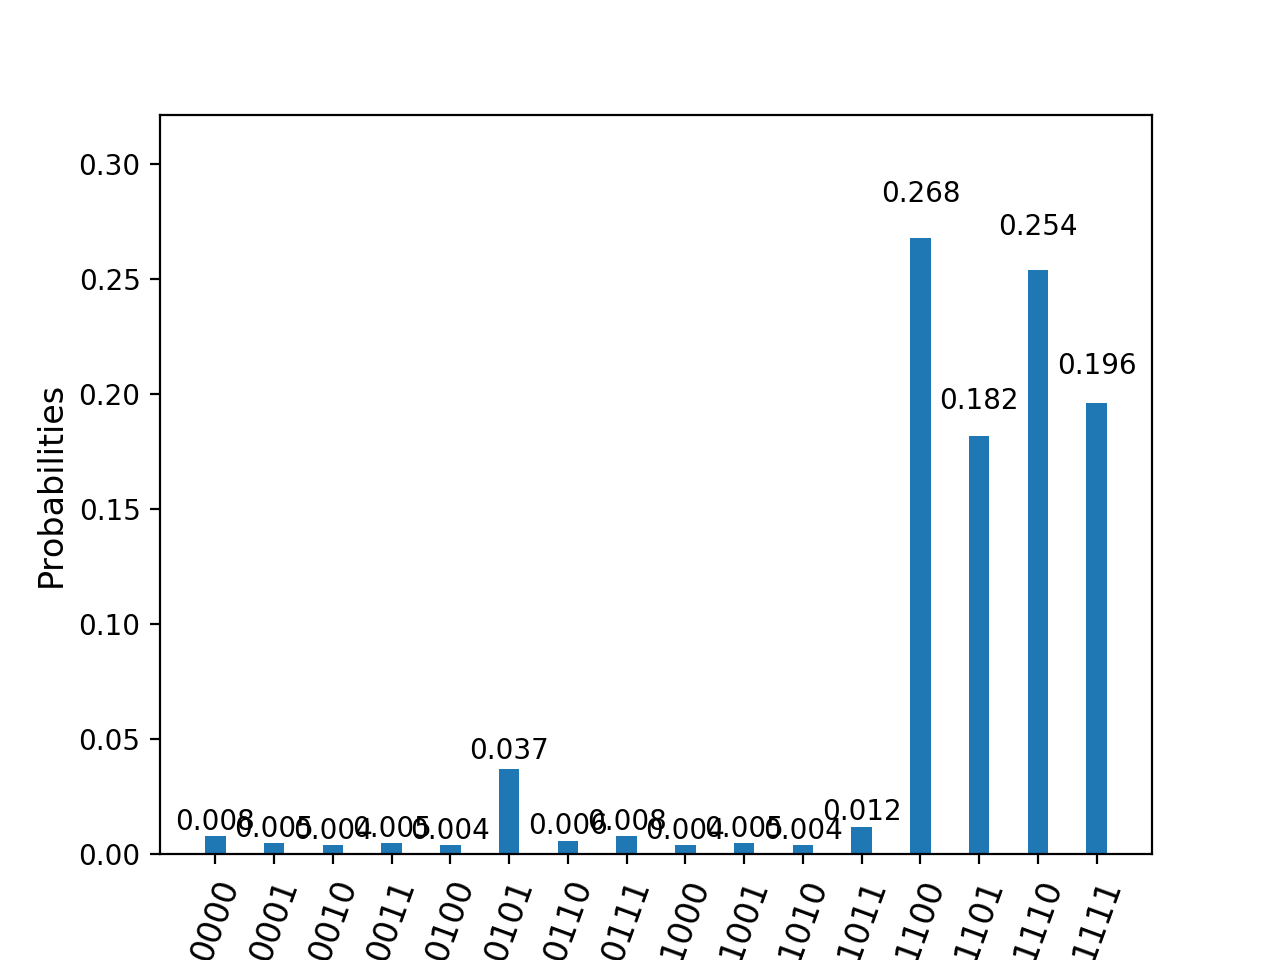
\includegraphics[scale=.55]{./3_sat.png}
	\end{figure}
\end{frame}
% Placing a * after \section means it will not show in the
% outline or table of contents.
\section*{Summary}

\end{document}
